\documentclass[10pt,letterpaper,final,twoside,notitlepage]{article}
\usepackage[margin=.5in]{geometry} % 1/2 inch margins on all pages
\usepackage[utf8]{inputenc} % Define the input encoding
\usepackage[USenglish]{babel} % Define language used
\usepackage{amsmath,amsfonts,amssymb}
\usepackage{amsthm} % Gives us plain, definition, and remark to use in \theoremstyle{style}
\usepackage{mathtools} % Allow for text and math in align* environment.
\usepackage{thmtools}
\usepackage{thm-restate}
\usepackage{graphicx}

\usepackage[
backend=biber,
style=alphabetic,
citestyle=authoryear]{biblatex} % Must include citation somewhere in document to print bibliography
\usepackage{hyperref} % Generate hyperlinks to referenced items
\usepackage[nottoc]{tocbibind} % Prints the Reference/Bibliography in TOC as well
\usepackage[noabbrev,nameinlink]{cleveref} % Fancy cross-references in the document everywhere
\usepackage{nameref} % Can make references by name to places
\usepackage{caption} % Allows for greater control over captions in figure, algorithm, table, etc. environments
\usepackage{subcaption} % Allows for multiple figures in one Figure environment
\usepackage[binary-units=true]{siunitx} % Gives us ways to typeset units for stuff
\usepackage{csquotes} % Context-sensitive quotation facilities
\usepackage{enumitem} % Provides [noitemsep, nolistsep] for more compact lists
\usepackage{chngcntr} % Allows us to tamper with the counter a little more
\usepackage{empheq} % Allow boxing of equations in special math environments
\usepackage[x11names]{xcolor} % Gives access to coloring text in environments or just text, MUST be before tikz
\usepackage{tcolorbox} % Allows us to create boxes of various types for examples
\usepackage{tikz} % Allows us to create TikZ and PGF Pictures
\usepackage{ctable} % Greater control over tables and how they look
\usepackage{diagbox} % Allow us to have shared diagonal cells in tables
\usepackage{multirow} % Allow us to have a single cell in a table span multiple rows
\usepackage{titling} % Put document information throughout the document programmatically
\usepackage[linesnumbered,ruled,vlined]{algorithm2e} % Allows us to write algorithms in a nice style.

\counterwithin{figure}{section}
\counterwithin{table}{section}
\counterwithin{equation}{section}
\counterwithin{algocf}{section}
\crefname{algocf}{algorithm}{algorithms}
\Crefname{algocf}{Algorithm}{Algorithms}
\setcounter{secnumdepth}{4}
\setcounter{tocdepth}{4} % Include \paragraph in toc
\crefname{paragraph}{paragraph}{paragraphs}
\Crefname{paragraph}{Paragraph}{Paragraphs}

% Create a theorem environment
\theoremstyle{plain}
\newtheorem{theorem}{Theorem}[section]
% Create a numbered theorem-like environment for lemmas
\newtheorem{lemma}{Lemma}[theorem]

% Create a definition environment
\theoremstyle{definition}
\newtheorem{definition}{Defn}
\newtheorem{corollary}{Corollary}[section]
% \begin{definition}[Term] \label{def:}
%   Make sure the term is emphasized with \emph{term}.
%   This ensures that if \emph is changed, it shows up everywhere
% \end{definition}

% Create a numbered remark environment numbered based on definition
% NOTE: This version of remark MUST go inside a definition environment
\theoremstyle{remark}
\newtheorem{remark}{Remark}[definition]
%\counterwithin{definition}{subsection} % Uncomment to have definitions use section.subsection numbering

% Create an unnumbered remark environment for general use
% NOTE: This version of remark has NO restrictions on placement
\newtheorem*{remark*}{Remark}

% Create a special list that handles properties. It can be broken and restarted
\newlist{propertylist}{enumerate}{1} % {Name}{Template}{Max Depth}
% [newlistname, LevelsToApplyTo]{formatting options}
\setlist[propertylist, 1]{label=\textbf{(\roman*)}, ref=\textbf{(\roman*)}, noitemsep, nolistsep}
\crefname{propertylisti}{property}{properties}
\Crefname{propertylisti}{Property}{Properties}

% Create a special list that handles enumerate starting with lower letters. Breakable/Restartable.
\newlist{boldalphlist}{enumerate}{1} % {Name}{Template}{Max Depth}
% [newlistname, LevelsToApplyTo]{formatting options}
\setlist[boldalphlist, 1]{label=\textbf{(\alph*)}, ref=\alph*, noitemsep, nolistsep} % Set options

\newlist{nocrefenumerate}{enumerate}{1} % {Name}{Template}{Max Depth}
% [newlistname, LevelsToApplyTo]{formatting options}
\setlist[nocrefenumerate, 1]{label=(\arabic*), ref=(\arabic*), noitemsep, nolistsep}

% Create a list that allows for deeper nesting of numbers. By default enumerate only allows depth=4.
\newlist{nestednums}{enumerate}{6}
% [newlistname, LevelsToApplyTo]{formatting options}
\setlist[nestednums]{noitemsep, label*=\arabic*.}

\tcbuselibrary{breakable} % Allow tcolorboxes to be broken across pages
% Create a tcolorbox for examples
% /begin{example}[extra name]{NAME}
% Create a tcolorbox for examples
% Argument #1 is optional, given by [], that is the textbook's problem number
% Argument #2 is mandatory, given by {}, that is the title for the example
% Avoid putting special characters, (), [], {}, ",", etc. in the title.
\newtcolorbox[auto counter,
number within=section,
number format=\arabic,
crefname={example}{examples}, % Define reference format for cref (No Capitals)
Crefname={Example}{Examples}, % Reference format for cleveref (With Capitals)
]{example}[2][]{ % The [2][] Means the first argument is optional
  width=\textwidth,
  title={Example \thetcbcounter: #2. #1}, % Parentheses and commas are not well supported
  fonttitle=\bfseries,
  label={ex:#2},
  nameref=#2,
  colbacktitle=white!100!black,
  coltitle=black!100!white,
  colback=white!100!black,
  upperbox=visible,
  lowerbox=visible,
  sharp corners=all,
  breakable
}

% Create a tcolorbox for general use
\newtcolorbox[% auto counter,
% number within=section,
% number format=\arabic,
% crefname={example}{examples}, % Define reference format for cref (No Capitals)
% Crefname={Example}{Examples}, % Reference format for cleveref (With Capitals)
]{blackbox}{
  width=\textwidth,
  % title={},
  fonttitle=\bfseries,
  % label={},
  % nameref=,
  colbacktitle=white!100!black,
  coltitle=black!100!white,
  colback=white!100!black,
  upperbox=visible,
  lowerbox=visible,
  sharp corners=all
}

% Redefine the 'end of proof' symbol to be a black square, not blank
\renewcommand{\qedsymbol}{$\blacksquare$} % Change proofs to have black square at end

% Common Mathematical Stuff
\newcommand{\Abs}[1]{\ensuremath{\lvert #1 \rvert}}
\newcommand{\DNE}{\ensuremath{\mathrm{DNE}}} % Used when limit of function Does Not Exist

% Complex Numbers functions
\renewcommand{\Re}{\operatorname{Re}} % Redefine to use the command, but not the fraktur version
\renewcommand{\Im}{\operatorname{Im}} % Redefine to use the command, but not the fraktur version
\newcommand{\Real}[1]{\ensuremath{\Re \lbrace #1 \rbrace}}
\newcommand{\Imag}[1]{\ensuremath{\Im \lbrace #1 \rbrace}}
\newcommand{\Conjugate}[1]{\ensuremath{\overline{#1}}}
\newcommand{\Modulus}[1]{\ensuremath{\lvert #1 \rvert}}
\DeclareMathOperator{\PrincipalArg}{\ensuremath{Arg}}

% Math Operators that are useful to abstract the written math away to one spot
% Number Sets
\DeclareMathOperator{\RealNumbers}{\ensuremath{\mathbb{R}}}
\DeclareMathOperator{\AllIntegers}{\ensuremath{\mathbb{Z}}}
\DeclareMathOperator{\PositiveInts}{\ensuremath{\mathbb{Z}^{+}}}
\DeclareMathOperator{\NegativeInts}{\ensuremath{\mathbb{Z}^{-}}}
\DeclareMathOperator{\NaturalNumbers}{\ensuremath{\mathbb{N}}}
\DeclareMathOperator{\ComplexNumbers}{\ensuremath{\mathbb{C}}}
\DeclareMathOperator{\RationalNumbers}{\ensuremath{\mathbb{Q}}}

% Calculus operators
\DeclareMathOperator*{\argmax}{argmax} % Thin Space and subscripts are UNDER in display

% Signal and System Functions
\DeclareMathOperator{\UnitStep}{\mathcal{U}}
\DeclareMathOperator{\sinc}{sinc} % sinc(x) = (sin(pi x)/(pi x))

% Transformations
\DeclareMathOperator{\Lapl}{\mathcal{L}} % Declare a Laplace symbol to be used

% Logical Operators
\DeclareMathOperator{\XOR}{\oplus}

% x86 CPU Registers
\newcommand{\rbpRegister}{\texttt{\%rbp}}
\newcommand{\rspRegister}{\texttt{\%rsp}}
\newcommand{\ripRegister}{\texttt{\%rip}}
\newcommand{\raxRegister}{\texttt{\%rax}}
\newcommand{\rbxRegister}{\texttt{\%rbx}}

%%% Local Variables:
%%% mode: latex
%%% TeX-master: shared
%%% End:


% These packages are more specific to certain documents, but will be availabe in the template
% \usepackage{esint} % Provides us with more types of integral symbols to use
% \usepackage[outputdir=./TeX_Output]{minted} % Allow us to nicely typeset 300+ programming languages
% \crefname{lstlisting}{listing}{listings}
% \Crefname{lstlisting}{Listing}{Listings}
% This document must be compiled with the -shell-escape flag if the packages above are uncommented

\sisetup{per-mode=symbol}

\DeclareSymbolFont{matha}{OML}{txmi}{m}{it} % txfonts
\DeclareMathSymbol{\DriftVelocity}{\mathord}{matha}{118} % A more angled v

\graphicspath{{./Drawings/ECE_311-Engineering_Electronics/}} % Uncomment this to use pictures in this document
\addbibresource{./Bibliographies/ECE_311-Engineering_Electronics.bib}
% % Define English Imperial units.
% Length
\DeclareSIUnit\inch{in}
\DeclareSIUnit\in{in}

\DeclareSIUnit\feet{ft}
\DeclareSIUnit\ft{ft}

\DeclareSIUnit\yard{yd}
\DeclareSIUnit\yd{yd}

\DeclareSIUnit\mile{mi}
\DeclareSIUnit\mi{mi}

% Volume
\DeclareSIUnit\fluidOunce{fl oz}
\DeclareSIUnit\floz{fl oz}

\DeclareSIUnit\pint{pt}
\DeclareSIUnit\pt{pt}

\DeclareSIUnit\quart{qt}
\DeclareSIUnit\qt{qt}

\DeclareSIUnit\gallon{gal}
\DeclareSIUnit\gal{gal}

% Mass
\DeclareSIUnit\grain{gr}
\DeclareSIUnit\gr{gr}

\DeclareSIUnit\ounce{oz}
\DeclareSIUnit\oz{oz}

\DeclareSIUnit\pound{lb}
\DeclareSIUnit\lb{lb}

\DeclareSIUnit\poundMass{lbm}
\DeclareSIUnit\lbm{lbm}

\DeclareSIUnit\ton{t}
\DeclareSIUnit\slug{slug}

% Temperature
\DeclareSIUnit\rankine{R}
\DeclareSIUnit[number-unit-product={}]\degreeF{\degree{}F}
\DeclareSIUnit[number-unit-product={}]\dF{\degree{}F}
\DeclareSIUnit[number-unit-product={}]\degF{\degree{}F}

\DeclareSIUnit[number-unit-product={}]\degreeR{\degree{}R}
\DeclareSIUnit[number-unit-product={}]\dR{\degree{}R}
\DeclareSIUnit[number-unit-product={}]\degR{\degree{}R}
% \DeclareSIUnit[number-unit-product={}]\Rankine{\degree{}R}
% \DeclareSIUnit[number-unit-product={}]\rankine{\degree{}R}
\DeclareSIUnit[number-unit-product={}]\degreeRankine{\degree{}R}

% Pressure
\DeclareSIUnit\bar{bar}
\DeclareSIUnit\atm{atm}
\DeclareSIUnit\psia{psia}
\DeclareSIUnit\psig{psig}
\DeclareSIUnit\psi{psi}

% Energy
\DeclareSIUnit\btu{btu}
\DeclareSIUnit\BTU{BTU}

%Force
\DeclareSIUnit\poundForce{lbf}
\DeclareSIUnit\lbf{lbf}

% volumetric flow
\DeclareSIUnit\cfm{cfm}
\DeclareSIUnit\CFM{CFM}

% Moles
\DeclareSIUnit\lbmol{lbmol}

%%% Local Variables:
%%% mode: latex
%%% TeX-master: shared
%%% End:


% Math Operators that are useful to abstract the written math away to one spot
% These are supposed to be document-specific mathematical operators that will make life easier
% Many fundamental operators are defined in Reference_Sheet_Preamble.tex
\newcommand{\Temp}{\ensuremath{T}}
\newcommand{\BandgapEnergy}{\ensuremath{E_{g}}}
\newcommand{\BoltzmannConstant}{\ensuremath{k}}

\newcommand{\HoleConcentration}{\ensuremath{p}}
\newcommand{\HoleMobility}{\ensuremath{\mu_{\HoleConcentration}}}
\newcommand{\ElectronConcentration}{\ensuremath{n}}
\newcommand{\ElectronMobility}{\ensuremath{\mu_{\ElectronConcentration}}}
\newcommand{\eCharge}{\ensuremath{q}}
\newcommand{\PNJunction}{\ensuremath{pn}-Junction}
\newcommand{\SiElectricPermittivity}{\ensuremath{\epsilon_{\mathrm{Si}}}}
\newcommand{\JunctionBuiltInVoltage}{\ensuremath{V_{0}}}
\newcommand{\DepletionDistance}{\ensuremath{W}}
\newcommand{\AcceptorConcentration}{\ensuremath{N_{A}}}
\newcommand{\DonorConcentration}{\ensuremath{N_{D}}}

\begin{titlepage}
  \title{ECE 311: Engineering Electronics --- Reference Sheet \\ Illinois Institute of Technology}
  \author{Karl Hallsby}
  \date{Last Edited: \today} % We want to inform people when this document was last edited
\end{titlepage}

\begin{document}
\pagenumbering{gobble}
\maketitle
\pagenumbering{roman} % i, ii, iii on beginning pages, that don't have content
\tableofcontents
\clearpage
\listoftheorems[ignoreall, show={definition, Definition}]
\clearpage
\pagenumbering{arabic} % 1,2,3 on content pages

\section{Operational Amplifiers}\label{sec:Op-Amps}
\begin{definition}[Op-Amp]\label{def:Op-Amp}
  An \emph{op-amp}, (\emph{operational amplifier}), is a active circuit element that is a 2-port network element.
  An circuit symbol for an op-amp is shown in \Cref{fig:Op-Amp}.
\end{definition}


%%% Local Variables:
%%% mode: latex
%%% TeX-master: "../ECE_311-Engineering_Electronics-Reference_Sheet"
%%% End:


\section{Semiconductors}\label{sec:Semiconductors}
\subsection{Intrinsic Semiconductors}\label{subsec:Intrinsic_Semiconductors}
\begin{definition}[Semiconductor]\label{def:Semiconductor}
  \emph{Semiconductor}s are materials whose conductivity is somewhere between that of true conductors, like copper, and insulators, such as glass.
  Because semiconductors are somewhere between conductors and insulators, they have electrical properties that are easily manipulated through \nameref{def:Doping}.
\end{definition}

\begin{definition}[Electron]\label{def:Electron}
  An \emph{electron} in this scenario is a \textbf{free electron}.
  This means the electron is not bound to any particular atomic nucleus.
  Such an electron is free to conduct electric current if an electric field is applied.

  If an atom is missing electrons due to an electron being free, a \nameref{def:Hole} can be thought of in its place.
\end{definition}

The concentration of free \nameref{def:Electron}s in a material is given the symbol shown in \Cref{eq:Concentration_Free_Electrons}.

\begin{equation}\label{eq:Concentration_Free_Electrons}
  \ElectronConcentration
\end{equation}

\begin{definition}[Hole]\label{def:Hole}
  A \emph{hole} is the lack of an \nameref{def:Electron} being attached to an atom.
  These have the same, but opposite charge of an electron.

  \textbf{These are NOT particles in any physical sense}.
  Holes are useful abstractions to use when thinking about current flow in a semiconductor's crystal lattice.
\end{definition}

The concentration of free \nameref{def:Hole}s in a material is given the symbol shown in \Cref{eq:Concentration_Holes}.

\begin{equation}\label{eq:Concentration_Holes}
  \HoleConcentration
\end{equation}

\begin{definition}[Intrinsic]\label{def:Intrinsic}
  An \emph{intrinsic} material is one that is pure.
  It has a regular lattice structure, where atoms are held in place by covalent bonds.
\end{definition}

In an \nameref{def:Intrinsic} material, the concentration of free \nameref{def:Electron}s and \nameref{def:Hole}s are equal.
This is represented by the relation in \Cref{eq:Electron_Hole_Concentration-Intrinsic}.

\begin{equation}\label{eq:Electron_Hole_Concentration-Intrinsic}
  \ElectronConcentration = \HoleConcentration = \HoleElectronConcentration
\end{equation}

Typically, we express the product of \nameref{def:Hole} and free \nameref{def:Electron} concentrations as a product, shown in \Cref{eq:Electron_Hole_Concentration}.

\begin{equation}\label{eq:Electron_Hole_Concentration}
  \HoleConcentration \ElectronConcentration = \HoleElectronConcentration^{2}
\end{equation}

Semiconductor physics tells us that \HoleElectronConcentration{} is defined by \Cref{eq:Hole_Electron_Concentration}.
\begin{equation}\label{eq:Hole_Electron_Concentration}
  \HoleElectronConcentration = B \Temp^{\frac{3}{2}} e^{\frac{-\BandgapEnergy}{2 \BoltzmannConstant \Temp}}
\end{equation}

where
\begin{description}[noitemsep]
\item $B$ is a material-dependent parameter.
\item $\Temp$ is the temperature
\item $\BoltzmannConstant$ is Boltzmann's constant.
\end{description}

\subsection{Doped Semiconductors}\label{subsec:Doped_Semiconductors}
\begin{definition}[Doping]\label{def:Doping}
  \emph{Doping} is the process of deliberately adding atomic impurities to alter the electrical/conductivity characteristics of \nameref{def:Semiconductor}s.
  This is done by substantially increasing the concentration of \nameref{def:Electron}s or \nameref{def:Hole}s, but without changing the crystal properties of the original semiconductor.
\end{definition}

There are two kinds of doping:
\begin{enumerate}[noitemsep]
\item \ElectronConcentration{} Type.
  This is done by doping with an element with 5 valence electrons, typically phosphorus.
\item \HoleConcentration{} Type.
  This is done by doping with an element with 3 valence electrons, typically boron.
\end{enumerate}

If the concentration of donor atoms in an \ElectronConcentration{}-type doped \nameref{def:Semiconductor} is \DonorConcentration{}, where \DonorConcentration{} is much greater than \HoleElectronConcentration{} ($\DonorConcentration \gg \HoleConcentration$), then the concentration of \textbf{free \nameref{def:Electron}s} is:
\begin{equation}\label{eq:n-Type_Donor_Concentration}
  \ElectronConcentration_{\NType} \simeq \DonorConcentration
\end{equation}

By substituting \Cref{eq:n-Type_Donor_Concentration} into \Cref{eq:Hole_Electron_Concentration}, we can find the \nameref{def:Hole} concentration for an \ElectronConcentration{}-type \nameref{def:Semiconductor}.
\begin{equation}\label{eq:n-Type_Acceptor_Concentration}
  \HoleConcentration_{\NType} \simeq \frac{\HoleElectronConcentration^{2}}{\DonorConcentration}
\end{equation}

In an \NType-type doped \nameref{def:Semiconductor}, the free \nameref{def:Electron}s have a significantly larger concentration, and are said to be the \textbf{majority charge carriers}.
The \nameref{def:Hole}s are the \textbf{minority charge carriers}.

\begin{blackbox}
  The complete opposite of this holds true for \PType{}-type doped \nameref{def:Semiconductor}s.
  Meaning,
  \begin{equation*}
    \HoleConcentration_{\PType} \simeq \AcceptorConcentration
  \end{equation*}
  \begin{equation*}
    \ElectronConcentration_{\PType} \simeq \frac{\HoleElectronConcentration^{2}}{\AcceptorConcentration}
  \end{equation*}

  Similarly oppositely, in an \PType-type doped \nameref{def:Semiconductor}, the free \nameref{def:Hole}s have a significantly larger concentration, and are said to be the \textbf{majority charge carriers}.
The free \nameref{def:Electron}s are the \textbf{minority charge carriers}.
\end{blackbox}

\subsection{Current Flow in Semiconductors}\label{subsec:Semiconductors_Current_Flow}
\subsubsection{Drift Current}\label{subsubsec:Drift_Current}
\begin{definition}[Drift Current]\label{def:Drift_Current}
  \emph{Drift current} arises when an electric field \EField{} is applied to a \nameref{def:Semiconductor}.
  The \nameref{def:Hole}s are accelerated \textbf{in} the direction of \EField{}, and the free \nameref{def:Electron}s are accelerated in the \textbf{opposite} direction of \EField{}.
\end{definition}

In the presence of an electric field, because the drift current is made of of \nameref{def:Electron}s and \nameref{def:Hole}s moving due to a force field, they have a velocity.
This velocity is the \nameref{def:Drift_Velocity}.

\begin{definition}[Drift Velocity]\label{def:Drift_Velocity}
  \emph{Drift velocity} is the velocity that \nameref{def:Hole}s or \nameref{def:Electron}s gain when an electric field (voltage) is applied to the \nameref{def:Semiconductor}.
  There are two separate equations for drift velocity, one for \nameref{def:Hole}s and one for \nameref{def:Electron}s, shown in \Cref{eq:Drift_Velocity-Hole,eq:Drift_Velocity-Electron}, respectively.
\end{definition}

\begin{equation}\label{eq:Drift_Velocity-Hole}
  \DriftVelocity_{\HoleConcentration-\text{drift}} = \HoleMobility \EField
\end{equation}

\begin{equation}\label{eq:Drift_Velocity-Electron}
  \DriftVelocity_{\ElectronConcentration-\text{drift}} = -\ElectronMobility \EField
\end{equation}

\Cref{eq:Drift_Velocity-Electron} is negative because \nameref{def:Electron}s move in the opposite direction of the electric field \EField{}.

In \Cref{eq:Drift_Velocity-Hole,eq:Drift_Velocity-Electron}, the constants \HoleMobility{} and \ElectronMobility{} are used.
\HoleMobility{} is the \nameref{def:Hole_Mobility}.
\ElectronMobility{} is the \nameref{def:Electron_Mobility}.

\begin{definition}[Hole Mobility]\label{def:Hole_Mobility}
  \emph{Hole mobility}, \HoleMobility{} is a value representing how ``easy'' it is for \nameref{def:Hole}s to move through the \nameref{def:Semiconductor}'s crystal structure in response to an applied electric field, \EField{}.

  The hole mobility for \nameref{def:Intrinsic} silicon is a known constant, and is shown in \Cref{eq:Hole_Mobility-Intrinsic_Silicon}.
  \begin{equation}\label{eq:Hole_Mobility-Intrinsic_Silicon}
    \HoleMobility = \SI{480}{\centi\meter\squared\per\volt\per\second}
  \end{equation}
\end{definition}

\begin{definition}[Electron Mobility]\label{def:Electron_Mobility}
  \emph{Electron mobility}, \ElectronMobility{} is a value representing how ``easy'' it is for \nameref{def:Electron}s to move through the \nameref{def:Semiconductor}'s crystal structure in response to an applied electric field, \EField{}.

  The electron mobility for \nameref{def:Intrinsic} silicon is a known constant, and is shown in \Cref{eq:Electron_Mobility-Intrinsic_Silicon}.
  \begin{equation}\label{eq:Electron_Mobility-Intrinsic_Silicon}
    \ElectronMobility = \SI{1350}{\centi\meter\squared\per\volt\per\second}
  \end{equation}

  \begin{remark}
    \nameref{def:Electron}s move through a semiconductor's crystal lattice much more easily than \nameref{def:Hole}s do.
    This can be seen by $\ElectronMobility \approx 2.5 \HoleMobility$.
  \end{remark}
\end{definition}

We are interested in the current flowing through an object due to an applied electric field, so we use:
\begin{equation}\label{eq:Drift_Current-Hole}
  \DCCurrent{\HoleConcentration} = \Area \eCharge \HoleConcentration \DriftVelocity_{\HoleConcentration-\text{drift}}
\end{equation}

If we substitute $\DriftVelocity_{\HoleConcentration-\text{drift}}$ with our knowledge from \Cref{eq:Drift_Velocity-Hole}, then we have the equation below.

\begin{equation*}
  \DCCurrent{\HoleConcentration} = \Area \eCharge \HoleConcentration \HoleMobility \EField
\end{equation*}

If we divide this equation by the cross-sectional area, $\Area$, then we have \Cref{eq:Drift_Current_Density-Hole}.

\begin{equation}\label{eq:Drift_Current_Density-Hole}
  \CurrentDensity{\HoleConcentration} = \frac{\DCCurrent{\HoleConcentration}}{\Area} = \eCharge \HoleConcentration \HoleMobility \EField
\end{equation}

Similarly, we can find the drift current equation for $\DCCurrent{\ElectronConcentration}$ and the current density equation.

\begin{equation}\label{eq:Drift_Current-Electron}
  \DCCurrent{\ElectronConcentration} = - \Area \eCharge \ElectronConcentration \DriftVelocity_{\HoleConcentration-\text{drift}}
\end{equation}

\begin{equation}\label{eq:Drift_Current_Density-Electron}
  \CurrentDensity{\ElectronConcentration} = \eCharge \ElectronConcentration \ElectronMobility \EField
\end{equation}

Then the total drift current is just the addition of the two separate drift currents.

\begin{equation}\label{eq:Total_Drift_Current_Density}
  \CurrentDensity{} = \CurrentDensity{\HoleConcentration} + \CurrentDensity{\ElectronConcentration}
\end{equation}

By factoring out the constant terms, we end up with:
\begin{align*}
  \CurrentDensity{} &= \CurrentDensity{\HoleConcentration} + \CurrentDensity{\ElectronConcentration} \\
                    &= \eCharge \HoleConcentration \HoleMobility \EField + \eCharge \ElectronConcentration \ElectronMobility \EField \\
                    &= \eCharge (\HoleConcentration \HoleMobility + \ElectronConcentration \ElectronMobility) \EField \\
  \CurrentDensity{} &= \Conductivity \EField
\end{align*}

This leads to two important equations, \Cref{eq:Total_Current_Density-Conductivity,eq:Total_Current_Density-Resistivity}.

\begin{subequations}
  \begin{equation}\label{eq:Total_Current_Density-Conductivity}
    \CurrentDensity{} = \Conductivity \EField
  \end{equation}
  \begin{equation}\label{eq:Total_Current_Density-Resistivity}
    \CurrentDensity{} = \frac{\EField}{\Resistivity}
  \end{equation}
\end{subequations}

\subsubsection{Diffusion Current}\label{subsubsec:Diffusion_Current}
\begin{definition}[Diffusion Current]\label{def:Diffusion_Current}
  \emph{Diffusion current} arises due to concentration differences in \nameref{def:Electron}s and \nameref{def:Hole}s in a semiconductor.
\end{definition}

\subsection{The \PNJunction{} Junction}\label{subsec:The_pn_Junction}

\subsection{The \PNJunction{} Junction with Applied Voltage}\label{subsec:The_pn_Junction-Voltage_Applied}

\subsection{Depletion Layer}\label{subsec:Depletion_Layer}
\begin{definition}[Depletion Layer]\label{def:Depletion_Layer}
  The \emph{depletion layer} is the location in the \PNJunction{} where the two differently-doped sides meet.
  Here, there is a barrier of the opposing carrier on each side.
  This is visualized in \Cref{fig:Depletion_Layer}.
\end{definition}

\begin{figure}[h!tbp]
  \centering
  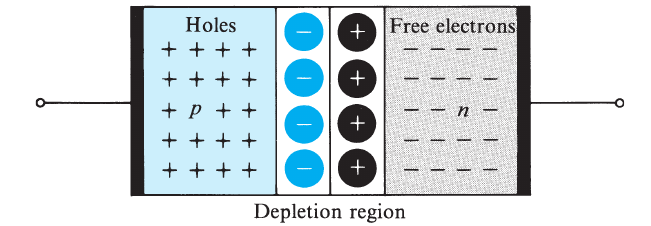
\includegraphics[scale=0.5]{./Depletion_Layer.png}
  \caption{Depletion Layer (\cite[p.~150]{sedraTextbook7})}
  \label{fig:Depletion_Layer}
\end{figure}

We can find the width of the \nameref{def:Depletion_Layer} using \Cref{eq:Depletion_Layer_Width}.
\begin{equation}\label{eq:Depletion_Layer_Width}
  \DepletionDistance = \sqrt{\frac{2 \SiElectricPermittivity}{\eCharge} \left( \frac{1}{\AcceptorConcentration} + \frac{1}{\DonorConcentration} \right) \JunctionBuiltInVoltage}
\end{equation}

The depletion layer ``bleeds'' into each side of the \PNJunction{}.
We can find the distance the depletion layer falls into each side with \Cref{eq:Depletion_Layer_Directions-Electron,eq:Depletion_Layer_Directions-Hole}.

\begin{subequations}\label{eq:Depletion_Layer_Directions}
  \begin{equation}\label{eq:Depletion_Layer_Directions-Electron}
    x_{\ElectronConcentration} = \DepletionDistance \left( \frac{\AcceptorConcentration}{\AcceptorConcentration + \DonorConcentration} \right)
  \end{equation}
  \begin{equation}\label{eq:Depletion_Layer_Directions-Hole}
    x_{\HoleConcentration} = \DepletionDistance \left( \frac{\DonorConcentration}{\AcceptorConcentration + \DonorConcentration} \right)
  \end{equation}
\end{subequations}

Lastly, the sum of the ``bleed'' in both directions is equal to the width of the entire \nameref{def:Depletion_Layer}.
\begin{equation}\label{eq:Depletion_Layer-Directions_Sum}
  \DepletionDistance = x_{\ElectronConcentration} + x_{\HoleConcentration}
\end{equation}

%%% Local Variables:
%%% mode: latex
%%% TeX-master: "../ECE_311-Engineering_Electronics-Reference_Sheet"
%%% End:


\section{Diodes}\label{sec:Diodes}
A \nameref{def:Diode} is one of the basic building blocks for almost all analog circuit systems.

\begin{definition}[Diode]\label{def:Diode}
  A \emph{diode} is a 2-port non-linear circuit element.
  Its circuit symbol is shown in \Cref{fig:Diode_Circuit_Symbol}.
\end{definition}

\begin{figure}[h!tbp]
  \centering
  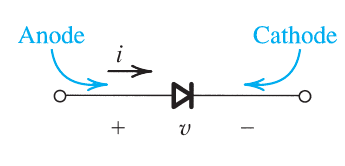
\includegraphics[scale=0.75]{./Diode_Circuit_Symbol.png}
  \caption{Diode Circuit Symbol \parencite[p.~177]{sedraTextbook7}}
  \label{fig:Diode_Circuit_Symbol}
\end{figure}

An \textbf{ideal diode} is one that behaves as a short-circuit when a voltage applied is forward-biased, and acts as an open-circuit with the voltage is reverse-biased.
The current-voltage characteristic is shown in \Cref{fig:Ideal_Diode_IV_Characteristic}.

\begin{figure}[h!tbp]
  \centering
  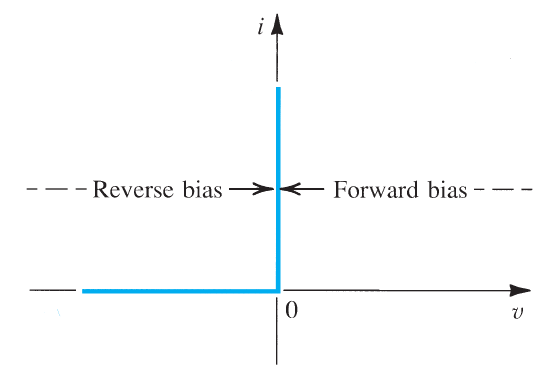
\includegraphics[scale=0.75]{./Ideal_Diode_IV_Characteristic.png}
  \caption{Ideal Diode \DCCurrent{}-\DCVoltage{} Characteristic \parencite[p.~177]{sedraTextbook7}}
  \label{fig:Ideal_Diode_IV_Characteristic}
\end{figure}

\subsection{Terminal Characteristics of Junction Diodes}\label{subsec:Terminal_Characteristics_Junction_Diodes}
A \textbf{junction diode} is a \nameref{def:Diode} built using a \PNJunction{}.
In this case, there are three distinct regions in the characteristic curve:
\begin{enumerate}[noitemsep]
\item \nameref{subsubsec:Diode_Forward-Bias_Region}, where $\Voltage > 0$.
\item \nameref{subsubsec:Diode_Reverse-Bias_Region}, where $\Voltage < 0$.
\item \nameref{subsubsec:Diode_Breakdown_Region}, where $\Voltage < - \ReverseBreakdownVoltage$.
\end{enumerate}

\subsubsection{The Forward-Bias Region}\label{subsubsec:Diode_Forward-Bias_Region}
The forward-bias region is the one where the terminal voltage $\Voltage$ is positive.

In the forward region, we can approximate the current-voltage relationship by using \Cref{eq:pn-Junction-Current-Voltage_Relation-Simple}, with minor modifications, as seen in \Cref{eq:Diode_Forward-Bias-IV_Relationship}.

\begin{equation}\label{eq:Diode_Forward-Bias-IV_Relationship}
  \Current = \SaturationCurrent \left( e^{\frac{\Voltage}{\ThermalVoltage}} - 1 \right)
\end{equation}

There is a slightly \textbf{more} modified version, in \Cref{eq:Diode_Forward-Bias-IV_Relationship-n}

\begin{equation}\label{eq:Diode_Forward-Bias-IV_Relationship-n}
  \Current = \SaturationCurrent \left( e^{\frac{\Voltage}{n \ThermalVoltage}} - 1 \right)
\end{equation}

$n$ has a value between 1 and 2.
$n$ is a number that depends on the material and physical structure of the diode.
From here-on-out, we assume that $n = 1$.
However, there may be cases when you should use a different $v$ value instead.

If the diode has $\Current \gg \SaturationCurrent$, then we can approximate \Cref{eq:Diode_Forward-Bias-IV_Relationship} using \Cref{eq:Diode_Forward-Bias-IV_Relationship-Approximate}.

\begin{equation}\label{eq:Diode_Forward-Bias-IV_Relationship-Approximate}
  \Current \simeq \SaturationCurrent e^{\frac{\Voltage}{\ThermalVoltage}}
\end{equation}

The relationship in \Cref{eq:Diode_Forward-Bias-IV_Relationship-Approximate} can be expressed in terms of currents instead of voltages as well.
\begin{equation}\label{eq:Diode_Forward-Bias-VI_Relationship-Approximate}
  \Voltage = \ThermalVoltage \ln \left( \frac{\Current}{\SaturationCurrent} \right)
\end{equation}

\subsubsection{The Reverse-Bias Region}\label{subsubsec:Diode_Reverse-Bias_Region}
In the reverse-bias region, the voltage applied to the \nameref{def:Diode} is in the reverse direction.
This causes the diode to behave \emph{like} an open-circuit.
However, this is not technically true, because a small amount of current does ``leak'' out, as seen by \Cref{eq:Diode_Reverse-Bias-Current_Relation}.

\begin{equation}\label{eq:Diode_Reverse-Bias-Current_Relation}
  \Current \simeq - \SaturationCurrent
\end{equation}

\subsubsection{The Breakdown Region}\label{subsubsec:Diode_Breakdown_Region}
Lastly, the breakdown region is where the voltage applied in the reverse-bias direction is so great, that the \nameref{def:Diode} starts working in reverse, conducting current in the reverse direction.
This region will be discussed much more in the section devoted to \nameref{subsec:Zener_Diodes}.

\subsection{Modeling the Diode's Forward Characteristic}\label{subsec:Modeling_Diode_Forward_Characteristic}
There are several different models, appropriate at different times of analysis.

\subsubsection{The Exponential Model}\label{subsubsec:Exponential_Diode_Model}
In the exponential model of a \nameref{def:Diode}, you use the diode's current-voltage characteristic and another equation containing the current through the diode and the voltage across the diode to solve for $\DCCurrent{D}$ and $\DCVoltage{D}$.

The downside to this model is that it can require a lot of knowledge about the \nameref{def:Diode} and its properties.
In addition, because an exponential function $\DCCurrent{D} = \SaturationCurrent e^{\frac{\DCVoltage{D}}{\ThermalVoltage}}$ and a linear function are being used to find a solution, finding that solution can be computationally difficult.
Due to this, it is only used in the final stages of circuit development/analysis and is not much discussed in either this document or this course.
Instead, we focus on ways to more quickly model a \nameref{def:Diode} and its characteristics.

\subsubsection{The Constant-Voltage-Drop Model}\label{subsubsec:Constant_Voltage_Drop_Diode_Model}
In the constant-voltage-drop model, we assume the \nameref{def:Diode} is semi-ideal.
Meaning that we approximate the real exponential function, $\DCCurrent{D} = \SaturationCurrent e^{\frac{\DCVoltage{D}}{\ThermalVoltage}}$ to a piecewise linear one.
The constant-voltage-drop model for a silicon-based diode is shown in \Cref{fig:Silicon_Diode_Constant_Voltage_Drop}.

\begin{figure}[h!tbp]
  \centering
  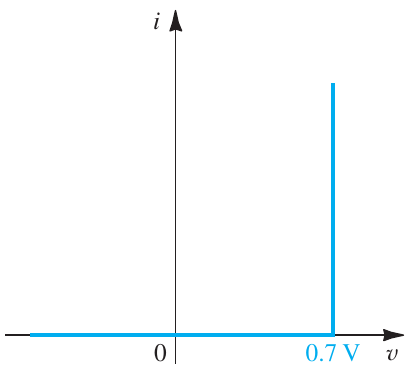
\includegraphics[scale=0.75]{./Silicon_Diode_Constant_Voltage_Drop}
  \caption{Silicon Diode Constant-Voltage-Drop Model \parencite[p.~193]{sedraTextbook7}}
  \label{fig:Silicon_Diode_Constant_Voltage_Drop}
\end{figure}

Essentially, this simplifies a \nameref{def:Diode} down to a DC voltage source, where the source's positive terminal is on the anode of the diode.
This source can then be used when performing circuit analysis to get reasonably accurate answers for the amount of work required.

\subsubsection{The Ideal Diode Model}\label{subsubsec:Ideal_Diode_Model}
In the ideal diode model, it is assumed that the \nameref{def:Diode} in question \textbf{is} ideal.
This means that if the voltage across the diode is greater than zero, the diode acts as a short-circuit.
This can be seen graphically in \Cref{fig:Ideal_Diode_IV_Characteristic}.

\subsubsection{The Small-Signal Model}\label{subsubsec:Diode_Small-Signal_Model}
In the small-signal model, we are interested in how small changes across the \nameref{def:Diode} affect its properties.
For example, say we increase the original source voltage $\Voltage_{S}$ by $\Delta \Voltage_{DD}$, we would be interested in the change in the diode's current and voltage.

To solve this, we actually use the exponential model, but we are only concerned with the highest one or two orders in the infinite summation.

\begin{blackbox}
  Remember that Euler's exponential can be represented using an infinite series, seen below:
  \begin{align*}
    e^{x} &= 1 + x + \frac{x^{2}}{2!} + \frac{x^{3}}{3!} + \cdots \\
    &= \sum\limits_{k = 0}^{\infty} \frac{x^{k}}{k!}
  \end{align*}
\end{blackbox}

If we are working with a small enough change ($\Delta \Voltage_{DD} \ll \ThermalVoltage$), then the exponential curve is dominated by the $1+x$ term in the infinite series.

To simplify the explanations here, we will pretend that the $\Delta \Voltage_{DD}$ is actually an AC voltage, $\ACVoltage{d}(t)$.

\begin{align*}
  \intertext{Then, by the theory of superposition, the voltage across the diode is also a time-varying function shown below.}
  \ACVoltage{D}(t) &= \DCVoltage{D} + \ACVoltage{d}(t) \\
  \intertext{Knowing how a \nameref{def:Diode} works, we can say,}
  \ACCurrent{D}(t) &= \SaturationCurrent e^{\frac{\ACVoltage{D}}{\ThermalVoltage}} \\
  \shortintertext{Substitute for $\ACVoltage{D}(t)$} \\
                   &= \SaturationCurrent e^{\frac{\DCVoltage{D} + \ACVoltage{d}(t)}{\ThermalVoltage}} \\
                   &= \SaturationCurrent e^{\frac{\DCVoltage{D}}{\ThermalVoltage}} e^{\frac{\ACVoltage{d}(t)}{\ThermalVoltage}} \\
  \intertext{Let $\DCCurrent{D} = \SaturationCurrent e^{\frac{\DCVoltage{D}}{\ThermalVoltage}}$.}
  \ACCurrent{D}(t) &= \DCCurrent{D} e^{\frac{\ACVoltage{d}(t)}{\ThermalVoltage}} \\
  \intertext{If we keep the amplitude of the change we introduce remain small, meaning the $e^{\frac{\ACVoltage{d}(t)}{\ThermalVoltage}} \approx 1$, then we can solve this.
  Such a constraint means that $\frac{\ACVoltage{d}(t)}{\ThermalVoltage} \ll 1$.
  Expanding the exponential using its infinite series and truncating after two terms yields a reasonable approximation.
  In that case:}
  \ACCurrent{D}(t) &\simeq \DCCurrent{D} \left( 1 + \frac{\ACVoltage{d}(t)}{\ThermalVoltage} \right) \\
\end{align*}


%%% Local Variables:
%%% mode: latex
%%% TeX-master: "../ECE_311-Engineering_Electronics-Reference_Sheet"
%%% End:


\section{MOS Field-Effect Transistors}\label{sec:MOSFETs}
In this section, we start studying \nameref{def:Transistor}s.

\begin{definition}[Transistor]\label{def:Transistor}
  A \emph{transistor} is a \nameref{def:Semiconductor} device used to amplify or switch electronic signals and electrical power.
  Transistors are one of the basic building blocks of modern electronics.
  It is composed of semiconductor material usually with at least three terminals for connection to an external circuit.
\end{definition}

The \nameref{def:MOSFET} is the first \nameref{def:Transistor} we will be studying in this course.
It is the second oldest transistor, but is the most frequently used one today, particularly for digital applications.

\begin{definition}[MOSFET]\label{def:MOSFET}
  \emph{MOSFET}, short for \emph{Metal-Oxide-\nameref{def:Semiconductor} Field-Effect \nameref{def:Transistor}}, is an insulated-gate field-effect transistor.

  The insulated-gate portion of its name implies that the gate is completely isolated from the rest of the circuit.
  This is achieved with the metal oxide layer (seen in \Cref{fig:MOSFET-Physical_Structure-Cross_Section}) acting as an insulator, preventing any current from entering the transistor from that terminal.

  The field-effect portion of the name implies that the electric field of the gate is the driving force in this circuit.
  Because no current is allowed through the gate terminal of the transistor, this only has a voltage applied, causing an electric field to form.

  The typical circuit symbol (for \nameref{def:NMOS}) is shown in \Cref{fig:MOSFET-Symbol-NMOS}.
\end{definition}

The physical structure of a \nameref{def:MOSFET} is shown in \Cref{fig:MOSFET-Physical_Structure-Perspective,fig:MOSFET-Physical_Structure-Cross_Section}.

\begin{figure}[h!tbp]
  \centering
  \begin{subfigure}[h!tbp]{0.48\linewidth}
    \centering
    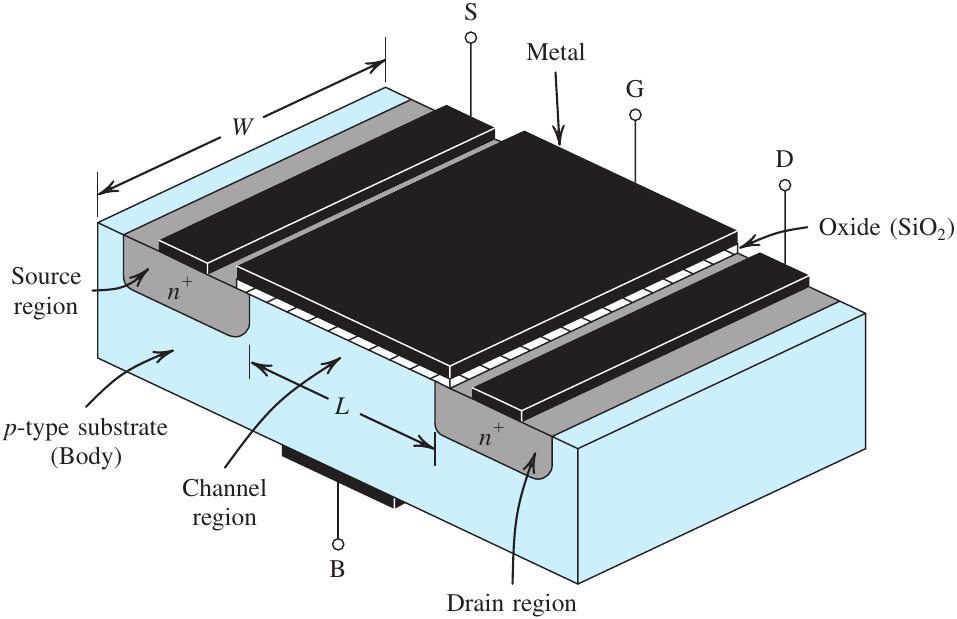
\includegraphics[scale=0.35]{./MOSFET-Physical_Structure-Perspective.png}
    \caption{Perspective View \parencite[p.~249]{sedraTextbook7}}
    \label{fig:MOSFET-Physical_Structure-Perspective}
  \end{subfigure}
  \begin{subfigure}[h!tbp]{0.48\linewidth}
    \centering
    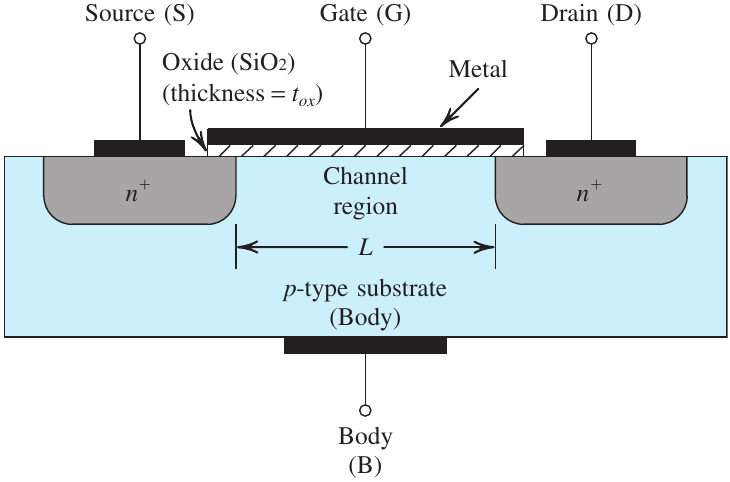
\includegraphics[scale=0.35]{./MOSFET-Physical_Structure-Cross_Section.png}
    \caption{Cross-Sectional View \parencite[p.~249]{sedraTextbook7}}
    \label{fig:MOSFET-Physical_Structure-Cross_Section}
  \end{subfigure}
  \caption{Physical Structure of Enhancement-type \nameref*{def:NMOS} \nameref*{def:Transistor}}
  \label{fig:MOSFET-Physical_Structure}
\end{figure}

As can be seen in \Cref{fig:MOSFET-Physical_Structure-Perspective}, the drain and source both form a \PNJunction{} with the base.

\subsection{No Gate Voltage}\label{subsec:MOSFET-No_Gate_Voltage}
When the gate has \textbf{no} voltage applied, the \PNJunction{}s of the source and drain to the substrate forms a diode-like relationship, where the resistance is very high (of the order $10^{12}\si{\ohm}$)
This prevents nearly all current from the drain from flowing.

\subsection{Gate Voltage Applied}\label{subsec:MOSFET-Gate_Voltage_Applied}
When the gate receives a positive voltage (in relation to the source), then an electric field is formed on the gate, causing a \nameref{def:Depletion_Layer} to form in the substrate.
Then, there is a channel that is formed due to the application of the electric field that allows current to flow between the drain and the source.
\Cref{fig:MOSFET-Gate_Voltage_Applied} shows this phenomena for \nameref{def:NMOS} \nameref{def:Transistor}s.

\begin{figure}[h!tbp]
  \centering
  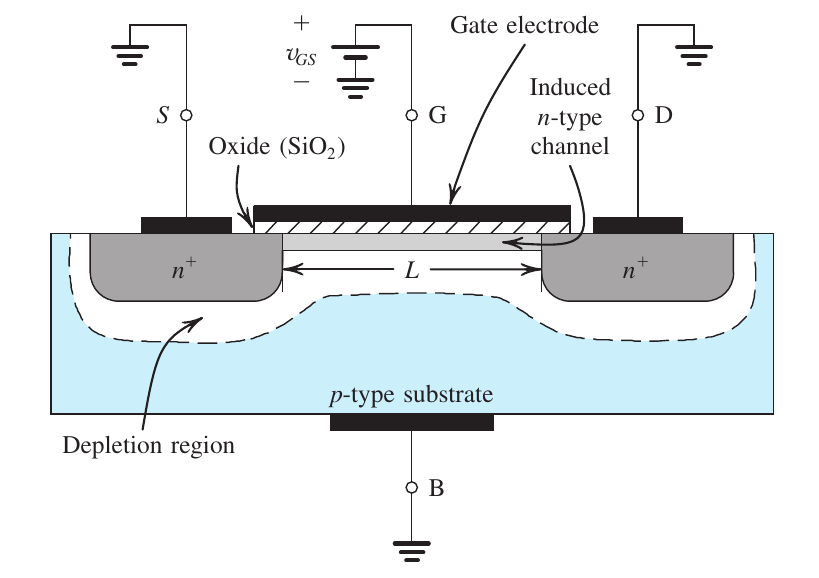
\includegraphics[scale=0.55]{./MOSFET-NMOS-Channel_Created.png}
  \caption{\nameref*{def:NMOS} \nameref*{def:MOSFET} with Positive Voltage Applied to Gate \parencite[p.~251]{sedraTextbook7}}
  \label{fig:MOSFET-Gate_Voltage_Applied}
\end{figure}

\begin{definition}[NMOS]\label{def:NMOS}
  \emph{NMOS}, short for \emph{\Channel{n} Metal-Oxide \nameref{def:Semiconductor}}.
  An \Channel{n} \nameref{def:MOSFET} is formed in a \PType{} substrate, and the induced channel is of \PType{}.
  The channel is created by inverting the substrate surface from \PType{} to \NType{}.
  Hence the induced channel is also called an \emph{inversion layer}.

  The circuit symbol for an NMOS transistor is shown in \Cref{fig:MOSFET-Symbol-NMOS}.
\end{definition}

\begin{figure}[h!tbp]
  \centering
  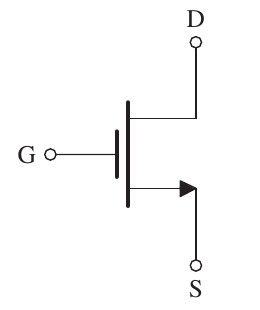
\includegraphics[scale=0.75]{./MOSFET-Symbol-NMOS.png}
  \caption{\nameref*{def:NMOS} \nameref*{def:MOSFET} Circuit Symbol \parencite[p.~265]{sedraTextbook7}}
  \label{fig:MOSFET-Symbol-NMOS}
\end{figure}

\begin{definition}[PMOS]\label{def:PMOS}
  \emph{PMOS}, short for \emph{\Channel{p} Metal-Oxide \nameref{def:Semiconductor}}.
  An \Channel{p} \nameref{def:MOSFET} is formed in a \NType{} substrate, and the induced channel is of \PType{}.
  The channel is created by inverting the substrate surface from \NType{} to \PType{}.
  Hence the induced channel is also called an \emph{inversion layer}.

  The circuit symbol for a PMOS transistor is shown in \Cref{fig:MOSFET-Symbol-PMOS}.
  The physical structure of the PMOS transistor (\Cref{fig:MOSFET-Physical_Structure-PMOS}) is similar to the \nameref{def:NMOS}, which we have studied.
\end{definition}

\begin{figure}[h!tbp]
  \centering
  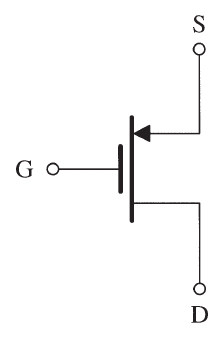
\includegraphics[scale=0.75]{./MOSFET-Symbol-PMOS.png}
  \caption{\nameref*{def:PMOS} \nameref*{def:MOSFET} Circuit Symbols \parencite[p.274]{sedraTextbook7}}
  \label{fig:MOSFET-Symbol-PMOS}
\end{figure}

\begin{figure}[h!tbp]
  \centering
  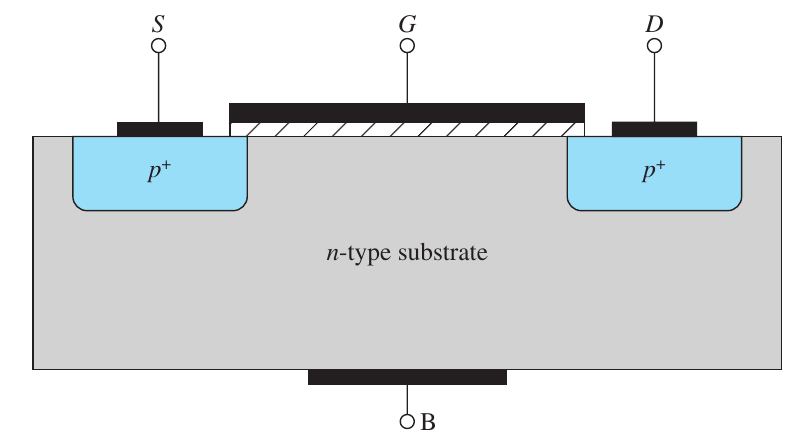
\includegraphics[scale=0.55]{./MOSFET-PMOS-Physical_Structure}
  \caption{\nameref*{def:PMOS} Physical Structure \parencite[p.~262]{sedraTextbook7}}
  \label{fig:MOSFET-Physical_Structure-PMOS}
\end{figure}

For such a channel to form, the voltage between the gate and the source, $\ACVoltage{\Gate\Source}$, \textbf{must} be greater than some \nameref{def:Threshold_Voltage}.

\begin{definition}[Threshold Voltage]\label{def:Threshold_Voltage}
  The \emph{threshold voltage} is a specific value for a \nameref{def:MOSFET} that determines the minimum required forltage that must be aplied at the gate for the transistor to operate.
  In this text, the threshold voltage is denoted as $\ThresholdVoltage$.

  \begin{remark}[Notation]
    Some materials use $\DCVoltage{T}$ as the \nameref{def:Threshold_Voltage}.
    We use $\ThresholdVoltage$, to distinguish this value from the \nameref{def:Thermal_Voltage}.
  \end{remark}
\end{definition}

If the gate-source voltage ($\ACVoltage{\Gate\Source}$) exceeds the \nameref{def:Threshold_Voltage}, we define a new term called \nameref{def:Overdrive_Voltage}.

\begin{definition}[Overdrive Voltage]\label{def:Overdrive_Voltage}
  The \emph{overdrive voltage} is the difference in voltage applied to the gate and the \nameref{def:Threshold_Voltage}.
  Its defining equation is given in \Cref{eq:Overdrive_Voltage}.

  \begin{equation}\label{eq:Overdrive_Voltage}
    \OverdriveVoltage = \ACVoltage{\Gate\Source} - \ThresholdVoltage
  \end{equation}
\end{definition}

If we leave the voltage at the drain (in relation to the source) equal to zero, then the channel has uniform depth in the \nameref{def:MOSFET}.

Because the gate and substrate are two parallel plates, separated by a dielectric, the plates function as a capacitor.
The capacitivity of the oxide is given by \Cref{eq:MOSFET-Oxide_Capacitivity}.

\begin{equation}\label{eq:MOSFET-Oxide_Capacitivity}
  \OxideCapacitivity = \frac{\OxidePermittivity}{\OxideThickness} \:\: \si{\farad\per\meter\squared}
\end{equation}

The magnitude of the total electron charge in the channel can be found using \Cref{eq:MOSFET-Oxide_Electron_Charge}.

\begin{equation}\label{eq:MOSFET-Oxide_Electron_Charge}
  \Magnitude{\Charge} = \OxideCapacitivity \OxideWidth \OxideLength \OverdriveVoltage
\end{equation}

To simplify many of our calculations, we use the terms shown in \Cref{eq:MOSFET-kPrime,eq:MOSFET-k}.
\begin{equation}\label{eq:MOSFET-kPrime}
  k_{n}' = \ElectronMobility \OxideCapacitivity
\end{equation}

\begin{equation}\label{eq:MOSFET-k}
  k = k_{n}' \left( \frac{\OxideWidth}{\OxideLength} \right)
\end{equation}

\begin{definition}[CMOS]\label{def:CMOS}
  \emph{CMOS}, or \emph{Complementary Metal-Oxide \nameref{def:Semiconductor}} is a \nameref{def:MOSFET} element that combines an \nameref{def:NMOS} and \nameref{def:PMOS} into a single package.

  \Cref{fig:MOSFET-Physical_Structure-CMOS} shows the physical structure of the CMOS transistor.
\end{definition}

\begin{figure}[h!tbp]
  \centering
  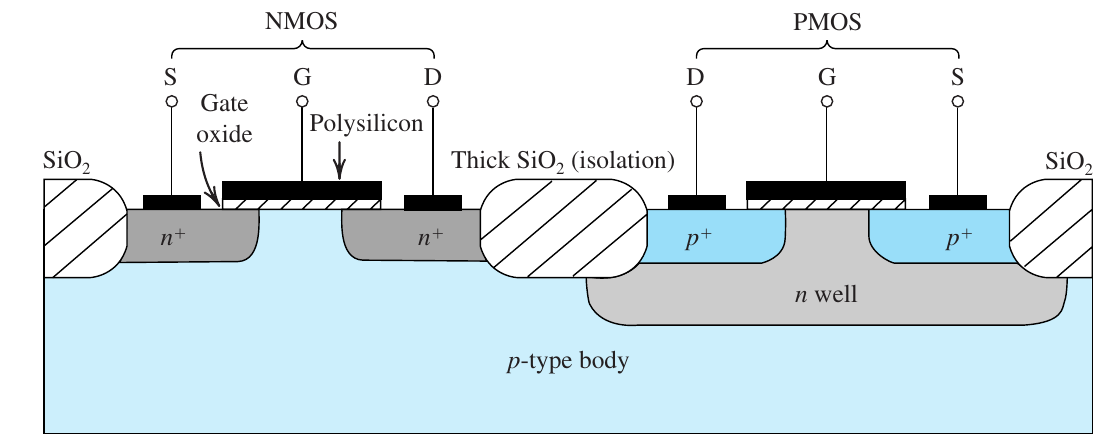
\includegraphics[scale=0.55]{./MOSFET-CMOS-Physical_Structure.png}
  \caption{\nameref*{def:CMOS} Transistor Physical Structure \parencite[p.~264]{sedraTextbook7}}
  \label{fig:MOSFET-Physical_Structure-CMOS}
\end{figure}

\subsection{Operating Regions}\label{subsec:MOSFET_Operating_Regions}
\nameref{def:MOSFET}s operate in one of three regions, based on two different voltages and their relationship.
\begin{enumerate}[noitemsep]
\item \nameref{subsubsec:MOSFET_Cutoff_Region}, $\DCVoltage{GS} < \ThresholdVoltage$
\item \nameref{subsubsec:MOSFET_Triode_Region}, $\DCVoltage{GS} \geq \ThresholdVoltage$ \textbf{and} $\DCVoltage{DS} < \OverdriveVoltage$
\item \nameref{subsubsec:MOSFET_Saturation_Region}, $\DCVoltage{GS} \geq \ThresholdVoltage$ \textbf{and} $\DCVoltage{DS} \geq \OverdriveVoltage$
\end{enumerate}

The current-voltage characteristic of the \nameref{def:NMOS} \nameref{def:MOSFET} is shown in \Cref{fig:MOSFET-Current_Voltage_Characteristic}.

\begin{figure}[h!tbp]
  \centering
  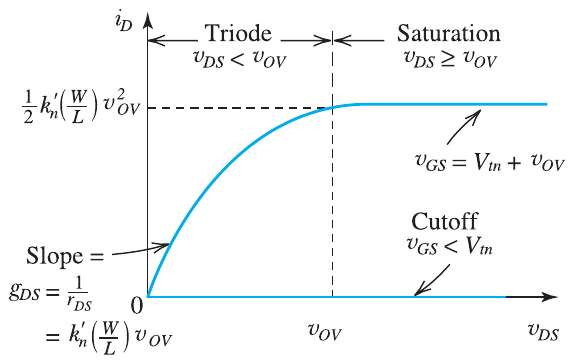
\includegraphics[scale=0.75]{./MOSFET-id_VDS.png}
  \caption{$\ACCurrent{\Drain}$-$\ACVoltage{\Drain\Source}$ \nameref*{def:NMOS} \nameref*{def:MOSFET} Characteristic \parencite[p.~266]{sedraTextbook7}}
  \label{fig:MOSFET-Current_Voltage_Characteristic}
\end{figure}

\subsubsection{Cutoff}\label{subsubsec:MOSFET_Cutoff_Region}
The cutoff region is when the voltage applied at the gate is not enough to make a channel form in the substrate of the \nameref{def:MOSFET}, meaning $\DCVoltage{\Gate\Source} < \ThresholdVoltage$.
Because no channel is formed, no current flows, thus the current is as defined in \Cref{eq:MOSFET_Cutoff_Region-Current}.

\begin{equation}\label{eq:MOSFET_Cutoff_Region-Current}
  \DCCurrent{D} = 0
\end{equation}


%%% Local Variables:
%%% mode: latex
%%% TeX-master: "../ECE_311-Engineering_Electronics-Reference_Sheet"
%%% End:


%====================================APPENDIX====================================
\appendix
\counterwithin{definition}{subsection}

\clearpage
\section{Complex Numbers}\label{sec:Complex_Numbers}
\begin{definition}[Complex Number]\label{def:Complex_Number}
  A \emph{complex number} is a hyper real number system.
  This means that two real numbers, $a, b \in \RealNumbers$, are used to construct the set of complex numbers, denoted $\ComplexNumbers$.

  A complex number is written, in Cartesian form, as shown in \Cref{eq:Complex_Number} below.
  \begin{equation}\label{eq:Complex_Number}
    z = a \pm ib
  \end{equation}
  where
  \begin{equation}\label{eq:Imaginary_Value}
    i = \sqrt{-1}
  \end{equation}

  \begin{remark*}[$i$ vs. $j$ for Imaginary Numbers]
    Complex numbers are generally denoted with either $i$ or $j$.
    Electrical engineering regularly makes use of $j$ as the imaginary value.
    This is because alternating current $i$ is already taken, so $j$ is used as the imaginary value instad.
  \end{remark*}
\end{definition}

\subsection{Parts of a Complex Number}\label{subsec:Complex_Number_Parts}
A \nameref{def:Complex_Number} is made of up 2 parts:
\begin{enumerate}[noitemsep]
\item \nameref{def:Real_Part}
\item \nameref{def:Imaginary_Part}
\end{enumerate}

\begin{definition}[Real Part]\label{def:Real_Part}
  The \emph{real part} of an imaginary number, denoted with the $\Re$ operator, is the portion of the \nameref{def:Complex_Number} with no part of the imaginary value $i$ present.

  If $z = x + iy$, then
  \begin{equation}\label{eq:Real_Part}
    \Real{z} = x
  \end{equation}

  \begin{remark}[Alternative Notation]\label{rmk:Real_Part_Alternative_Notation}
    The \nameref{def:Real_Part} of a number sometimes uses a slightly different symbol for denoting the operation.
    It is:
    \begin{equation*}
      \mathfrak{Re}
    \end{equation*}
  \end{remark}
\end{definition}

\begin{definition}[Imaginary Part]\label{def:Imaginary_Part}
  The \emph{imaginary part} of an imaginary number, denoted with the $\Im$ operator, is the portion of the \nameref{def:Complex_Number} where the imaginary value $i$ is present.

  If $z = x + iy$, then
  \begin{equation}\label{eq:Imaginary_Part}
    \Imag{z} = y
  \end{equation}

  \begin{remark}[Alternative Notation]\label{rmk:Imaginary_Part_Alternative_Notation}
    The \nameref{def:Imaginary_Part} of a number sometimes uses a slightly different symbol for denoting the operation.
    It is:
    \begin{equation*}
      \mathfrak{Im}
    \end{equation*}
  \end{remark}
\end{definition}

\subsection{Binary Operations}\label{subsec:Binary_Operations}

%%% Local Variables:
%%% mode: latex
%%% TeX-master: shared
%%% End:


\subsection{Complex Conjugates}\label{app:Complex_Conjugates}
\begin{definition}[Complex Conjugate]\label{def:Complex_Conjugate}
  The conjugate of a complex number is called its \emph{complex conjugate}.
  The complex conjugate of a complex number is the number with an equal real part and an imaginary part equal in magnitude but opposite in sign.
  If we have a complex number as shown below,
  \begin{equation*}
    z = a \pm bi
  \end{equation*}

  then, the conjugate is denoted and calculated as shown below.
  \begin{equation}\label{eq:Complex_Conjugates}
    \Conjugate{z} = a \mp bi
  \end{equation}
\end{definition}

The \nameref{def:Complex_Conjugate} can also be denoted with an asterisk ($*$).
This is generally done for complex functions, rather than single variables.
\begin{equation}\label{eq:Complex_Conjugates_Asterisk}
  z^{*} = \Conjugate{z}
\end{equation}

%%% Local Variables:
%%% mode: latex
%%% TeX-master: shared
%%% End:


\subsection{Geometry of Complex Numbers}\label{subsec:Geometry_Complex_Numbers}
So far, we have viewed \nameref{def:Complex_Number}s only algebraically.
However, we can also view them geometrically as points on a 2 dimensional \nameref{def:Argand_Plane}.

\begin{definition}[Argand Plane]\label{def:Argand_Plane}
  An \emph{Argane Plane} is a standard two dimensional plane whose points are all elements of the complex numbers, $z \in \ComplexNumbers$.
  This is taken from Descarte's definition of a completely real plane.

  The Argand plane contains 2 lines that form the axes, that indicate the real component and the imaginary component of the complex number specified.
\end{definition}

A \nameref{def:Complex_Number} can be viewed as a point in the \nameref{def:Argand_Plane}, where the \nameref{def:Real_Part} is the ``$x$''-component and the \nameref{def:Imaginary_Part} is the ``$y$''-component.

By plotting this, you see that we form a right triangle, so we can find the hypotenuse of that triangle.
This hypotenuse is the distance the point $p$ is from the origin, refered to as the \nameref{def:Complex_Number_Modulus}.
\begin{remark*}
  When working with \nameref{def:Complex_Number}s geometrically, we refer to the points, where they are defined like so:
  \begin{equation*}
    z = x + iy = p(x, y)
  \end{equation*}

  Note that $p$ is \textbf{not} a function of $x$ and $y$.
  Those are the values that inform us \textbf{where} $p$ is located on the \nameref{def:Argand_Plane}.
\end{remark*}

\subsubsection{Modulus of a Complex Number}\label{subsubsec:Complex_Number_Modulus}
\begin{definition}[Modulus]\label{def:Complex_Number_Modulus}
  The \emph{modulus} of a \nameref{def:Complex_Number} is the distance from the origin to the complex point $p$.
  This is based off the Pythagorean Theorem.
  \begin{equation}\label{eq:Complex_Number_Modulus}
    \begin{aligned}
      {\lvert z \rvert}^{2} = x^{2} + y^{2} &= z \Conjugate{z} \\
      \lvert z \rvert &= \sqrt{x^{2} + y^{2}}
    \end{aligned}
  \end{equation}
\end{definition}

\begin{propertylist}
\item The \emph{Law of Moduli} states that $\lvert z w \rvert = \lvert z \rvert \lvert w \rvert$.\label{prop:Law_of_Moduli}.
\end{propertylist}

We can prove \Cref{prop:Law_of_Moduli} using an algebraic identity.
\begin{proof}[Prove \Cref*{prop:Law_of_Moduli}]
  Let $z$ and $w$ be complex numbers ($z, w \in \ComplexNumbers$).
  We are asked to prove
  \begin{equation*}
    \lvert z w \rvert = \lvert z \rvert \lvert w \rvert
  \end{equation*}

  But, it is actually easier to prove
  \begin{equation*}
    {\lvert z w \rvert}^{2} = {\lvert z \rvert}^{2} {\lvert w \rvert}^{2}
  \end{equation*}

  We start by simplifying the ${\lvert z w \rvert}^{2}$ equation above.
  \begin{align*}
    {\lvert z w \rvert}^{2} &= {\lvert z \rvert}^{2} {\lvert w \rvert}^{2} \\
    \intertext{Using the definition of the \nameref{def:Complex_Number_Modulus} of a \nameref{def:Complex_Number} in \Cref{eq:Complex_Number_Modulus}, we can expand the modulus.}
                            &= (z w) (\Conjugate{z w}) \\
    \intertext{Using \Cref{prop:Complex_Conjugate_Split} for multiplication allows us to do the next step.}
                            &= (z w) (\Conjugate{z} \Conjugate{w}) \\
    \intertext{Using Multiplicative Associativity and Multiplicative Commutativity, we can simplify this further.}
                            &= (z \Conjugate{z}) (w \Conjugate{w}) \\
                            &= {\lvert z \rvert}^{2} {\lvert w \rvert}^{2}
  \end{align*}

  Note how we never needed to define $z$ or $w$, so this is as general a result as possible.
\end{proof}

\paragraph{Algebraic Effects of the Modulus' \Cref*{prop:Law_of_Moduli}}\label{par:Law_of_Moduli-Algebraic_Effects}
For this section, let $z = x_{1} + iy_{1}$ and $w = x_{2} + iy_{2}$.
Now,
\begin{align*}
  z w &= (x_{1}x_{2} - y_{1}y_{2}) + i(x_{1}y_{2} + x_{2}y_{1}) \\
  {\lvert z w \rvert}^{2} &= {(x_{1}x_{2} - y_{1}y_{2})}^{2} + {(x_{1}y_{2} + x_{2}y_{1})}^{2} \\
      &= \left( x_{1}^{2} + x_{2}^{2} \right) \left( x_{2}^{2} + y_{2}^{2} \right) \\
      &= {\lvert z \rvert}^{2} {\lvert w \rvert}^{2}
\end{align*}

However, the Law of Moduli (\Cref{prop:Law_of_Moduli}) does \textbf{not} hold for a hyper complex number system one that uses 2 or more imaginaries, i.e.\ $z = a + iy + jz$.
But, the Law of Moduli (\Cref{prop:Law_of_Moduli}) \textbf{does} hold for hyper complex number system that uses 3 imaginaries, $a = z + iy + jz + k \ell$.

\paragraph{Conceptual Effects of the Modulus' \Cref*{prop:Law_of_Moduli}}\label{par:Law_of_Moduli-Conceptual_Effects}
We are interested in seeing if $\lvert z w \rvert = (x_{1}^{2} + y_{1}^{2})(x_{2}^{2}+y_{2}^{2})$ can be extended to more complex terms (3 terms in the complex number).

However, Langrange proved that the equation below \textbf{always} holds.
Note that the $z$ below has no relation to the $z$ above.
\begin{equation*}
  (x_{1} + y_{1} + z_{1}) \neq X^{2} + Y^{2} + Z^{2}
\end{equation*}

%%% Local Variables:
%%% mode: latex
%%% TeX-master: shared
%%% End:


\subsection{Circles and Complex Numbers}\label{subsec:Circles_Complex_Numbers}
We need to define both a center and a radius, just like with regular purely real values.
\Cref{eq:Circles_Complex_Numbers} defines the relation required for a circle using \nameref{def:Complex_Number}s.
\begin{equation}\label{eq:Circles_Complex_Numbers}
  \lvert z - a \rvert = r
\end{equation}

\begin{example}[Lecture 2, Example 1]{Convert to Circle}
  Given the expression below, find the location of the center of the circle and the radius of the circle?
  \begin{equation*}
    \lvert 5 iz + 10 \rvert = 7
  \end{equation*}
  \tcblower{}
  This is just a matter of simplification and moving terms around.
  \begin{align*}
    \lvert 5 iz + 10 \rvert &= 7 \\
    \lvert 5i (z + \frac{10}{5i}) \rvert &= 7 \\
    \lvert 5i (z + \frac{2}{i}) \rvert &= 7 \\
    \lvert 5i (z + \frac{2}{i} \frac{-i}{-i}) \rvert &= 7 \\
    \lvert 5i (z - 2i) \rvert &= 7 \\
    \intertext{Now using the Law of Moduli (\Cref{prop:Law_of_Moduli}) $\lvert a b \rvert = \lvert a \rvert \lvert b \rvert$, we can simplify out the extra imaginary term.}
    \lvert 5i \rvert \lvert z-2i \rvert &= 7 \\
    5 \lvert z - 2i \rvert &= 7 \\
    \lvert z - 2i \rvert = \frac{7}{5}
  \end{align*}

  Thus, the circle formed by the equation $\lvert 5 iz + 10 \rvert = 7$ is actually $\lvert z - 2i \rvert = \frac{7}{5}$, with a center at $a = 2i$ and a radius of $\frac{7}{5}$.
\end{example}

\subsubsection{Annulus}\label{subsubsec:Annulus}
\begin{definition}[Annulus]\label{def:Annulus}
  An \emph{annulus} is a region that is bounded by 2 concentric circles.
  This takes the form of \Cref{eq:Annulus}.
  \begin{equation}\label{eq:Annulus}
    r_{1} \leq \lvert z - a \rvert \leq r_{2}
  \end{equation}

  In \Cref{eq:Annulus}, each of the $\leq$ symbols could also be replaced with $<$.
  This leads to 3 different possibilities for the annulus:
  \begin{enumerate}[noitemsep]
  \item If both inequality symbols are $\leq$, then it is a \textbf{Closed Annulus}.
  \item If both inequality symbols are $<$, then it is an \textbf{Open Annulus}.
  \item If \textbf{only one} inequality symbol $<$ and the other $\leq$, then it is not an \textbf{Open Annulus}.
  \end{enumerate}
\end{definition}


%%% Local Variables:
%%% mode: latex
%%% TeX-master: shared
%%% End:



%%% Local Variables:
%%% mode: latex
%%% TeX-master: shared
%%% End:

\clearpage
\subsection{Trigonometry} \label{app:Trig}
	\subsubsection{Trigonometric Formulas} \label{subsubsec:Trig Formulas}
		\begin{equation} \label{eq:Sin plus Sin with diff Angles}
			\sin \left( \alpha \right) + \sin \left( \beta \right) = 2 \sin \left( \frac{\alpha + \beta}{2} \right) \cos\left( \frac{\alpha - \beta}{2} \right)  
		\end{equation}
		\begin{equation} \label{eq:Cosine-Sine Product}
			\cos \left( \theta \right) \sin \left( \theta \right) = \frac{1}{2} \sin \left( 2 \theta \right)
		\end{equation}
	
	\subsubsection{Euler Equivalents of Trigonometric Functions} \label{subsubsec:Euler Equivalents}
		\begin{equation} \label{eq:Euler Sin}
			\sin \left( x \right) = \frac{e^{\imath x} + e^{-\imath x}}{2}
		\end{equation}
		\begin{equation} \label{eq:Euler Cos}
			\cos \left( x \right) = \frac{e^{\imath x} - e^{-\imath x}}{2 \imath}
		\end{equation}
		\begin{equation} \label{eq:Euler Sinh}
			\sinh \left( x \right) = \frac{e^{x} - e^{-x}}{2}
		\end{equation}
		\begin{equation} \label{eq:Euler Cosh}
			\cosh \left( x \right) = \frac{e^{x} + e^{-x}}{2}
		\end{equation}

\clearpage
\section{Calculus}\label{app:Calculus}
\subsection{L'Hopital's Rule}\label{subsec:LHopitals_Rule}
L'Hopital's Rule can be used to simplify and solve expressions regarding limits that yield irreconcialable results.
\begin{lemma}[L'Hopital's Rule]\label{lemma:LHopitals_Rule}
  If the equation
  \begin{equation*}
    \lim\limits_{x \rightarrow a} \frac{f(x)}{g(x)} =
    \begin{cases}
      \frac{0}{0} \\
      \frac{\infty}{\infty} \\
    \end{cases}
  \end{equation*}
  then \Cref{eq:LHopitals_Rule} holds.
  \begin{equation}\label{eq:LHopitals_Rule}
    \lim\limits_{x \rightarrow a} \frac{f(x)}{g(x)} = \lim\limits_{x \rightarrow a} \frac{f'(x)}{g'(x)}
  \end{equation}
\end{lemma}

\subsection{Fundamental Theorems of Calculus}\label{subsec:Fundamental Theorem of Calculus}
\begin{definition}[First Fundamental Theorem of Calculus]\label{def:1st Fundamental Theorem of Calculus}
  The \emph{first fundamental theorem of calculus} states that, if $f$ is continuous on the closed interval $\left[ a,b \right]$ and $F$ is the indefinite integral of $f$ on $\left[ a,b \right]$, then

  \begin{equation}\label{eq:1st Fundamental Theorem of Calculus}
    \int_{a}^{b}f \left( x \right) dx = F \left( b \right) - F \left( a \right)
  \end{equation}
\end{definition}

\begin{definition}[Second Fundamental Theorem of Calculus]\label{def:2nd Fundamental Theorem of Calculus}
  The \emph{second fundamental theorem of calculus} holds for $f$ a continuous function on an open interval $I$ and $a$ any point in $I$, and states that if $F$ is defined by

  \begin{equation*}
    F \left( x \right) = \int_{a}^{x} f \left( t \right) dt,
  \end{equation*}
  then
  \begin{equation}\label{eq:2nd Fundamental Theorem of Calculus}
    \begin{aligned}
      \frac{d}{dx} \int_{a}^{x} f \left( t \right) dt &= f \left( x \right) \\
      F' \left( x \right) &= f \left( x \right) \\
    \end{aligned}
  \end{equation}
\end{definition}

\begin{definition}[argmax]\label{def:argmax}
  The arguments to the \emph{argmax} function are to be maximized by using their derivatives.
  You must take the derivative of the function, find critical points, then determine if that critical point is a global maxima.
  This is denoted as
  \begin{equation*}\label{eq:argmax}
    \argmax_{x}
  \end{equation*}
\end{definition}

\subsection{Rules of Calculus}\label{subsec:Rules of Calculus}
\subsubsection{Chain Rule}\label{subsubsec:Chain Rule}
\begin{definition}[Chain Rule]\label{def:Chain Rule}
  The \emph{chain rule} is a way to differentiate a function that has 2 functions multiplied together.

  If
  \begin{equation*}
    f(x) = g(x) \cdot h(x)
  \end{equation*}
  then,
  \begin{equation}\label{eq:Chain Rule}
    \begin{aligned}
      f'(x) &= g'(x) \cdot h(x) + g(x) \cdot h'(x) \\
      \frac{df(x)}{dx} &= \frac{dg(x)}{dx} \cdot g(x) + g(x) \cdot \frac{dh(x)}{dx} \\
    \end{aligned}
  \end{equation}
\end{definition}

\subsection{Useful Integrals}\label{subsec:Useful_Integrals}
\begin{equation}\label{eq:Cosine_Indefinite_Integral}
  \int \cos(x) \; dx = \sin(x)
\end{equation}

\begin{equation}\label{eq:Sine_Indefinite_Integral}
  \int \sin(x) \; dx = -\cos(x)
\end{equation}

\begin{equation}\label{eq:x_Cosine_Indefinite_Integral}
  \int x \cos(x) \; dx = \cos(x) + x \sin(x)
\end{equation}
\Cref{eq:x_Cosine_Indefinite_Integral} simplified with Integration by Parts.

\begin{equation}\label{eq:x_Sine_Indefinite_Integral}
  \int x \sin(x) \; dx = \sin(x) - x \cos(x)
\end{equation}
\Cref{eq:x_Sine_Indefinite_Integral} simplified with Integration by Parts.

\begin{equation}\label{eq:x_Squared_Cosine_Indefinite_Integral}
  \int x^{2} \cos(x) \; dx = 2x \cos(x) + (x^{2} - 2) \sin(x)
\end{equation}
\Cref{eq:x_Squared_Cosine_Indefinite_Integral} simplified by using Integration by Parts twice.

\begin{equation}\label{eq:x_Squared_Sine_Indefinite_Integral}
  \int x^{2} \sin(x) \; dx = 2x \sin(x) - (x^{2} - 2) \cos(x)
\end{equation}
\Cref{eq:x_Squared_Sine_Indefinite_Integral} simplified by using Integration by Parts twice.

\begin{equation}\label{eq:Exponential_Cosine_Indefinite_Integral}
  \int e^{\alpha x} \cos(\beta x) \; dx = \frac{e^{\alpha x} \bigl( \alpha \cos(\beta x) + \beta \sin(\beta x) \bigr)}{\alpha^{2} + \beta^{2}} + C
\end{equation}

\begin{equation}\label{eq:Exponential_Sine_Indefinite_Integral}
  \int e^{\alpha x} \sin(\beta x) \; dx = \frac{e^{\alpha x} \bigl( \alpha \sin(\beta x) - \beta \cos(\beta x) \bigr)}{\alpha^{2}+\beta^{2}} + C
\end{equation}

\begin{equation}\label{eq:Exponential_Indefinite_Integral}
  \int e^{\alpha x} \; dx = \frac{e^{\alpha x}}{\alpha}
\end{equation}

\begin{equation}\label{eq:x_Exponential_Indefinite_Integral}
  \int x e^{\alpha x} \; dx = e^{\alpha x} \left( \frac{x}{\alpha} - \frac{1}{\alpha^{2}} \right)
\end{equation}
\Cref{eq:x_Exponential_Indefinite_Integral} simplified with Integration by Parts.

\begin{equation}\label{eq:Inverse_x_Indefinite_Integral}
  \int \frac{dx}{\alpha + \beta x} = \int \frac{1}{\alpha + \beta x} \; dx = \frac{1}{\beta} \ln (\alpha + \beta x)
\end{equation}

\begin{equation}\label{eq:Inverse_x_Squared_Indefinite_Integral}
  \int \frac{dx}{\alpha^{2} + \beta^{2} x^{2}} = \int \frac{1}{\alpha^{2} + \beta^{2} x^{2}} \; dx = \frac{1}{\alpha \beta} \arctan \left( \frac{\beta x}{\alpha} \right)
\end{equation}

\begin{equation}\label{eq:a_Exponential_Indefinite_Integral}
  \int \alpha^{x} \; dx = \frac{\alpha^{x}}{\ln(\alpha)}
\end{equation}

\begin{equation}\label{eq:a_Exponential_Derivative}
  \frac{d}{dx} \alpha^{x} = \frac{d\alpha^{x}}{dx} = \alpha^{x} \ln(x)
\end{equation}

\subsection{Leibnitz's Rule}\label{subsec:Leibnitzs_Rule}
\begin{lemma}[Leibnitz's Rule]\label{lemma:Leibnitzs_Rule}
  Given
  \begin{equation*}
    g(t) = \int_{a(t)}^{b(t)} f(x, t) \, dx
  \end{equation*}
  with $a(t)$ and $b(t)$ differentiable in $t$ and $\frac{\partial f(x, t)}{\partial t}$ continuous in both $t$ and $x$, then
  \begin{equation}\label{eq:Leibnitzs_Rule}
    \frac{d}{dt} g(t) = \frac{d g(t)}{dt} = \int_{a(t)}^{b(t)} \frac{\partial f(x, t)}{\partial t} \, dx + f \bigl[ b(t), t \bigr] \, \frac{d b(t)}{dt} - f \bigl[ a(t), t \bigr] \, \frac{d a(t)}{dt}
  \end{equation}
\end{lemma}



\clearpage
\section{Laplace Transform}\label{app:Laplace_Transform}
\subsection{Laplace Transform}\label{subsec:Laplace_Transform}
\begin{definition}[Laplace Transform]\label{def:Laplace_Transform}
  The \emph{Laplace transformation} operation is denoted as $\Lapl \lbrace x(t) \rbrace$ and is defined as
  \begin{equation}\label{eq:Laplace_Transform}
    X(s) = \int\limits_{-\infty}^{\infty} x(t) e^{-st} dt
  \end{equation}
\end{definition}

\subsection{Inverse Laplace Transform}\label{subsec:Inverse_Laplace_Transform}
\begin{definition}[Inverse Laplace Transform]\label{def:Inverse_Laplace_Transform}
  The \emph{inverse Laplace transformation} operation is denoted as $\Lapl^{-1} \lbrace X(s) \rbrace$ and is defined as
  \begin{equation}\label{eq:Inverse_Laplace_Transform}
    x(t) = \frac{1}{2j \pi} \int_{\sigma-\infty}^{\sigma+\infty} X(s) e^{st} \, ds
  \end{equation}
\end{definition}

\subsection{Properties of the Laplace Transform}\label{subsec:Laplace_Transform_Properties}
\subsubsection{Linearity}\label{subsubsec:Laplace_Linearity}
The \nameref{def:Laplace_Transform} is a linear operation, meaning it obeys the laws of linearity.
This means \Cref{eq:Laplace_Linearity} must hold.
\begin{subequations}\label{eq:Laplace_Linearity}
  \begin{equation}\label{eq:Laplace_Linearity_Time}
    x(t) = \alpha_{1} x_{1}(t) + \alpha_{2} x_{2}(t)
  \end{equation}
  \begin{equation}\label{eq:Laplace_Linearity_Frequency}
    X(s) = \alpha_{1} X_{1}(s) + \alpha_{2} X_{2}(s)
  \end{equation}
\end{subequations}

\subsubsection{Time Scaling}\label{subsubsec:Laplace_Time_Scaling}
Scaling in the time domain (expanding or contracting) yields a slightly different transform.
However, this only makes sense for $\alpha > 0$ in this case.
This is seen in \Cref{eq:Laplace_Time_Scaling}.
\begin{equation}\label{eq:Laplace_Time_Scaling}
  \Lapl \bigl\lbrace x(\alpha t) \bigr\rbrace = \frac{1}{\alpha} X \left( \frac{s}{\alpha} \right)
\end{equation}

\subsubsection{Time Shift}\label{subsubsec:Laplace_Time_Shift}
Shifting in the time domain means to change the point at which we consider $t=0$.
\Cref{eq:Laplace_Time_Shifting} below holds for shifting both forward in time and backward.
\begin{equation}\label{eq:Laplace_Time_Shifting}
  \Lapl \bigl\lbrace x(t-a) \bigr\rbrace = X(s) e^{-a s}
\end{equation}

\subsubsection{Frequency Shift}\label{subsubsec:Laplace_Frequency_Shift}
Shifting in the frequency domain means to change the complex exponential in the time domain.
\begin{equation}\label{eq:Laplace_Frequency_Shift}
  \Lapl^{-1} \bigl\lbrace X(s-a) \bigr\rbrace = x(t)e^{at}
\end{equation}

\subsubsection{Integration in Time}\label{subsubsec:Laplace_Time_Integration}
Integrating in time is equivalent to scaling in the frequency domain.
\begin{equation}\label{eq:Laplace_Time_Integration}
  \Lapl \left\lbrace \int_{0}^{t} x(\lambda) \, d\lambda \right\rbrace = \frac{1}{s} X(s)
\end{equation}

\subsubsection{Frequency Multiplication}\label{subsubsec:Laplace_Frequency_Multiplication}
Multiplication of two signals in the frequency domain is equivalent to a convolution of the signals in the time domain.
\begin{equation}\label{eq:Laplace_Frequency_Multiplication}
  \Lapl \bigl\lbrace x(t) * v(t) \bigr\rbrace = X(s) V(s)
\end{equation}

\subsubsection{Relation to Fourier Transform}\label{subsubsec:Fourier_Transform_Relation}
The Fourier transform looks and behaves very similarly to the Laplace transform.
In fact, if $X(\omega)$ exists, then \Cref{eq:Fourier_Laplace_Transform_Relation} holds.
\begin{equation}\label{eq:Fourier_Laplace_Transform_Relation}
  X(s) = X(\omega) \vert_{\omega = \frac{s}{j}}
\end{equation}

\subsection{Theorems}\label{subsec:Laplace_Theorems}
There are 2 theorems that are most useful here:
\begin{enumerate}[noitemsep]
\item \nameref{thm:Laplace_Initial_Value_Theorem}
\item \nameref{thm:Laplace_Final_Value_Theorem}
\end{enumerate}


%%% Local Variables:
%%% mode: latex
%%% TeX-master: shared
%%% End:


% To make this print, you must include a citation somewhere in the document
\clearpage
\printbibliography{}
\end{document}